
\chapter{Inference for categorical data}
\label{inferenceForCategoricalData}

Statistical inference is concerned primarily with understanding the
accuracy of parameter estimates. While the equations and details change
depending on the setting, the foundations for inference are the same
throughout all of statistics. We introduce these common themes in
Sections~\ref{pointEstimates}-\ref{hypothesisTesting} by discussing
inference about the population proportion, $p$.
In Sections~\ref{}-\ref{}, we'll expand
to the application of comparing two proportions against each other.
Finally, we'll complete this chapter by analyzing categorical data
where there are many levels.

Each of the ideas in this chapter are applicable to a broad set of
applications and new contexts. We'll expand on these ideas in later
chapters.


%__________________
\section[Point estimates and sampling variability]{Point
    estimates and sampling variability} %\sectionvideohref{youtube-DNIauUrRIEM&list=PLkIselvEzpM7Pjo94m1e7J5jkIZkbQAl4}~\sectionslideshref{gdoc_os3_slides_4-1}}
\label{pointEstimates}

\index{data!solar survey|(}

\newcommand{\pewsolarpollsize}{1000}
\newcommand{\pewsolarpollprop}{0.887}
\newcommand{\pewsolarpollpropcomplement}{0.113}
\newcommand{\pewsolarpollpercent}{88.7}
\newcommand{\pewsolarpollpercentcomplement}{11.3}
\newcommand{\pewsolarpollcount}{887}
\newcommand{\pewsolarpollcountcomplement}{113}
\newcommand{\pewsolarpollse}{0.0100}

Pew Research conducted a poll in 2018 gauging public opinion of
American adults on solar and wind energy. They surveyed 1,000
Americans and found that \pewsolarpollpercent{}\% of respondents
favored expanding
solar energy.\footnote{The full survey's sample size was 2541,
and we've taken a subsample. To find the survey details, see\\
\oiRedirect{textbook-pew_2018_poll_on_solar_and_wind_expansion}{http://www.pewinternet.org/2018/05/14/majorities-see-government-efforts-to-protect-the-environment-as-insufficient}}
\Comment{The redirect link in the footnote needs to be confirmed as
working.}
One of the most common questions people ask about polls is
\begin{quote}
If the poll was based on only a couple thousand people, how reliable is it?
\end{quote}
If we took another poll, we wouldn't get the exact same answer.
Ultimately, it's unlikely that the actual proportion of Americans
who support expanding solar energy is \emph{exactly}
\pewsolarpollpercent{}\%, but it's probably something close to
\pewsolarpollpercent{}\%.

In this section, we discuss what a point estimate like
\pewsolarpollpercent{}\% represents
and the uncertainty associated with such an estimate. We'll also
be using some new notation and terminology:
\begin{itemize}
\item The population proportion will be written as $p$, which
    is called a \term{parameter} of the population. In the solar
    survey, $p$ represents the proportion of \emph{all}
    American adults who support solar energy. It's rare
    that we know the parameter. Instead, we often
    take a sample and compute an estimate.
\item Using Pew Research sample, we can estimate that the proportion
    of American adults who support expanding solar energy is
    \pewsolarpollpercent{}\%.
    This is called the \term{sample proportion}, and it gets a special
    label of $\hat{p}$ (spoken as \emph{p-hat}).
\item The \termsub{size of a sample}{sample size} will generally
    be denoted by $n$. In the case of this Pew Research poll,
    $n = \pewsolarpollsize{}$.
\end{itemize}

\subsection{Point Estimates}

\index{point estimate|(}

The sample proportion $\hat{p} = \pewsolarpollprop{}$ is called
the \term{point estimate} of the parameter $p$, since based
on the sample, this is our single best estimate of $p$.

The poll provides a \term{point estimate} of the actual proportion
of American adults that support expanding solar energy.
This estimate of \pewsolarpollpercent{}\% is unlikely to be perfect,
and it's quite possible for the \term{true proportion}
(a.k.a. the population proportion) to be a little lower
or a little higher. The difference between a point estimate
and the parameter is called the estimate's \term{error}.

\Comment{Should we aggressively cut out the usage of ``true''
  in the way it is used above?}

The error varies from one sample to the next: maybe
in one sample it is 1\% too low while in another
it is 3\% too high. Unfortunately, we rarely know the direction
or size of the error in our estimates, so instead we focus
on understanding what kinds of errors are typical.


\subsection{Understanding the variability of a point estimate}
\label{simulationForUnderstandingVariabilitySection}

We want to understand \emph{how does the
sample proportion $\hat{p}$ behave when the population
proportion is about \pewsolarpollprop{}}. We could
run the survey again to see how consistent the results
are, but who has the time and money for that? Instead,
we can investigate the properties of $\hat{p}$ using simulations.

To simulate the sample, we'll suppose that the population
proportion is exactly \pewsolarpollpercent{}\%.
%Now, we know
%the population proportion isn't exactly \pewsolarpollpercent\%,
%but we do expect it to be close, so this simulation will offer
%us some insights about the property of $\hat{p}$.
%If we took a random sample
%from this population, how accurate would the point estimate be?
Here's how we might simulate it:
\begin{enumerate}
\item There were about 250 million American adults in 2018.
    On 250 million pieces of paper, write ``support''
    on \pewsolarpollpercent{}\% of them and ``not'' on
    the other \pewsolarpollpercentcomplement{}\%.
\item Mix up the pieces of paper and pull out \pewsolarpollsize{}
    pieces to represent our sample of 1000 American adults.
\item Compute the fraction of the sample that say ``support''.
\end{enumerate}
Any volunteers to conduct this simulation? Probably not. Running
this simulation with 250 million pieces of paper would be
time-consuming and very costly, but we can simulate it
using computer code; we've written a short program in the
footnote.\footnote{Code using the statistical software called \R: \\
\texttt{\# 1. Create a set of 250 million entries,
where 89\% of them are "support" and 11\% are "not". \\
possible\_entries <- rep(c("support", "not"),
    c(\pewsolarpollprop{}, \pewsolarpollpropcomplement{}) * 250e6)\\
\# 2. Sample \pewsolarpollsize{} of the entries. \\
sampled\_entries <- sample(possible\_entries, \pewsolarpollsize{}) \\
\# 3. Count the number that are "justified", then divide
by the sample size. \\
sum(sampled\_entries == "justified") / \pewsolarpollsize{}}}
In this simulation, the sample gave a point estimate of
$\hat{p}_1 = 0.901$. We~know the population proportion
in this simulation is $p = \pewsolarpollprop{}$, so we know
the estimate had an error of +0.014.

One simulation isn't enough to get a sense of the null
distribution, so we should run more simulations. In a second
simulation, we get $\hat{p}_2 = 0.892$, which has an error of
+0.005.
In another, $\hat{p}_3 = 0.885$ for an error of -0.002. And in another,
an estimate of $\hat{p}_4 = 0.866$ with an error of -0.021.
With the help of a computer, we've run the simulation 10,000 times
and created a histogram of the results from all 10,000 simulations
in Figure~\ref{sampling_10k_prop_887p}. This
distribution of sample proportions is called a
\term{sampling distribution}.
%\footnote{Here is the code for 10,000 simulations: \\
%\texttt{people <- rep(c("justified", "not"), c(0.56, 0.44) * 247e6) \\
%sim.results <- c() \\
%for (i in 1:10000) \{ \\
%\ \hspace{5mm}sampled.people <- sample(people, 1000) \\
%\ \hspace{5mm}sim.results[i] <- mean(sampled.people == "justified") \\
%\} \\
%hist(sim.results, 20)} \\
%(There's actually a more efficient way to write this code, but we have provided you the long version!)}
We can characterize this sampling distribution as follows:
\begin{description}
\item[Center.] The center of the distribution is
    $\bar{x}_{\hat{p}} = \pewsolarpollprop{}0$, which is the same as the
    population proportion.
    That~is, we see that the sample proportion is an
    \term{unbiased estimate} of the population proportion.
\item[Spread.] The standard deviation of the distribution
    is $s_{\hat{p}} = \pewsolarpollse{}$. When we're talking about
    a sampling distribution or the variability of
    a point estimate, we typically use the term
    \termsub{standard error}{standard error (SE)}
    rather than \emph{standard deviation},
    and the notation $SE_{\hat{p}}$ is used for the standard
    error associated with the sample proportion.
\item[Shape.] The distribution is symmetric and bell-shaped,
    and it \emph{resembles a normal distribution}.
\end{description}
These findings are very encouraging! When the population
proportion is $p = \pewsolarpollprop{}$ and the sample size is
$n = \pewsolarpollsize{}$,
the sample proportion $\hat{p}$ tends to give a pretty good estimate
of the population proportion. We also have this interesting observation
that the histogram resembles a normal distribution.

\begin{figure}
   \centering
   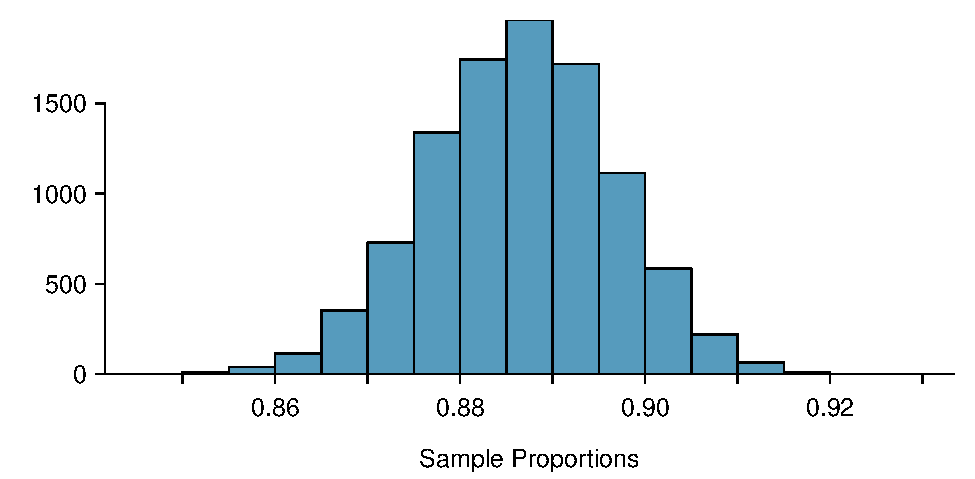
\includegraphics[width=0.8\textwidth]{ch_inference_for_props/figures/sampling_10k_prop_887p/sampling_10k_prop_887p}
   \caption{A histogram of 10,000 sample proportions, where each
       sample is taken from a population where the population of
       proportion is \pewsolarpollprop{} and the sample size is
       $n = \pewsolarpollsize{}$.}
   \label{sampling_10k_prop_887p}
\end{figure}

\begin{tipBox}{\tBoxTitle{Sampling distributions are something we
    keep in mind, even if they are never observed}
  In real-world applications, we never actually observe the
  sampling distribution, yet it is useful to always think of
  the sample proportion as coming from such a distribution.
  Understanding the distribution will help us characterize
  and make sense of the individual point estimate that we
  do observe.}
\end{tipBox}

\begin{example}{If we used a much smaller sample size of $n = 50$,
would you guess that the standard error for $\hat{p}$ would be larger
or smaller than when we used $n = \pewsolarpollsize{}$?}
\label{smallerSampleWhatHappensToPropErrorExercise}
Intuitively, it seems like more data is better
than less data, and generally that is correct! The typical error
when $p = \pewsolarpollprop{}$ and $n = 50$ would be larger
than the error we would expect when $n = \pewsolarpollsize{}$.
\end{example}

%\noindent
Example~\ref{smallerSampleWhatHappensToPropErrorExercise}
highlights an important property: a bigger sample
tends to provide a more precise point estimates than a smaller sample.

\index{point estimate|)}


\subsection{Central Limit Theorem}

The distribution in
Figure~\ref{sampling_10k_prop_887p} looks an awful lot like
a normal distribution. That is no anomaly; it is the result
of a general principle called the \term{Central Limit Theorem}.
\index{Central Limit Theorem!proportion|textbf}

\begin{termBox}{\tBoxTitle{Central Limit Theorem for proportions
    \& the success-failure condition}
When the observations are independent and the sample size is
sufficiently large, the sample proportion $\hat{p}$ will tend
to follow a normal distribution with the following mean and
standard error:
\begin{align*}
  \mu_{\hat{p}} &= p
  &SE_{\hat{p}} &= \sqrt{\frac{p (1 - p)}{n}}
\end{align*}
The sample size is typically considered sufficiently large when
$np \geq 10$ and $n(1-p) \geq 10$, which is called the
\term{success-failure condition}.} %since $np$ represents the
%number of expected \emph{successes} and $n(1-p)$ the expected
%number of \emph{failures}.}
\end{termBox}

The Central Limit Theorem is incredibly important, and it provides
a foundation for the rest of this book. As we begin applying
this principle, be mindful of the two requirements:
the observations must be independent, and the the sample size must
be sufficiently large such that $np \geq 10$ and $n(1-p) \geq 10$.

\begin{example}{Earlier we estimated the mean and standard
deviation of the $\hat{p}$'s using simulated data when
$p = \pewsolarpollprop{}$ and $n = \pewsolarpollsize{}$.
Confirm that the distribution is approximately
normal.}\label{sample_p887_n1000_confirm_normal}
\begin{description}
\item[Independence.] There are $n = \pewsolarpollsize{}$
    observations for each
    sample proportion $\hat{p}$, and each of those observations
    are independent draws. \emph{The most common way for
    observations to be considered independent is if they are from
    a simple random sample.}
    \index{independent}
    \index{independence}
    \index{Central Limit Theorem|independence}
\item[Success-failure condition.] We can confirm the sample size
    is sufficiently large by checking the success-failure condition
    and confirming each of the following values are greater than 10:
    \begin{align*}
    np &= \pewsolarpollsize{} \times \pewsolarpollprop{}
        = \pewsolarpollcount{}
    &n(1-p) &= \pewsolarpollsize{} \times (1 - \pewsolarpollprop{})
        = \pewsolarpollcountcomplement{}
    \end{align*}
\end{description}
Both of the independence and success-failure conditions are
satisfied, so the Central Limit Theorem applies and the normal
distribution is reasonable in this context!
\end{example}

\begin{example}{Compute the theoretical mean and standard deviation
of the $\hat{p}$'s when
$p = \pewsolarpollprop{}$ and $n = \pewsolarpollsize{}$,
according to the
Central Limit Theorem.}\label{sample_p887_n1000_mean_se}
The mean of the $\hat{p}$'s is simply the population proportion:
$\mu_{\hat{p}} = \pewsolarpollprop{}$.

The calculation of the standard error of $\hat{p}$ uses
the following formula:
\begin{align*}
SE_{\hat{p}}
    = \sqrt{\frac{p (1 - p)}{n}}
    = \sqrt{\frac{\pewsolarpollprop{} (1 - \pewsolarpollprop{})}{1000}}
    = \pewsolarpollse{}
\end{align*}
\end{example}

\begin{example}{Estimate how frequently the sample proportion
$\hat{p}$ should be within 0.02 (2\%) of the population value,
$p = \pewsolarpollprop{}$. Based on
Examples~\ref{sample_p887_n1000_confirm_normal}
and~\ref{sample_p887_n1000_mean_se}, we know that the distribution is
$N(\mu_{\hat{p}} = \pewsolarpollprop{}, SE_{\hat{p}} = \pewsolarpollse{})$.}
\label{sampling_10k_prop_887p-prop_from_867_to_907}
After so much practice in Section~\ref{normalDist},
this example will hopefully feel familiar!
We would like to understand the fraction of $\hat{p}$'s
between 0.867 and 0.907:
\begin{center}
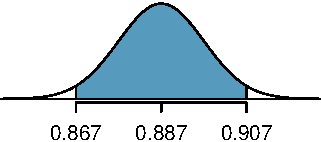
\includegraphics[width=60mm]{ch_inference_for_props/figures/p-hat_from_867_and_907/p-hat_from_867_and_907}
\end{center}
With $\mu_{\hat{p}} = \pewsolarpollprop{}$ and
$SE_{\hat{p}} = \pewsolarpollse{}$,
we can compute the Z-score for both the left and right cutoffs:
\begin{align*}
Z_{0.867} &= \frac{0.867 - \pewsolarpollprop{}}{\pewsolarpollse{}} = -2
&Z_{0.907} &= \frac{0.907 - \pewsolarpollprop{}}{\pewsolarpollse{}} = 2
\end{align*}
We can use either statistical software, a graphing calculator,
or a table to find the areas to the tails, and in any case we
will find that they are each 0.0228. The total tail areas are
$2 \times 0.0228 = 0.0456$, which leaves the shaded area of
0.9544. That is, about 95.44\% of the sampling distribution
in Figure~\ref{sampling_10k_prop_887p} is within $\pm0.02$
of the simulation population proportion, $p = \pewsolarpollprop{}$.
%of these
%cutoffs and compute the difference of these areas
%to get the central area:
%\begin{center}
%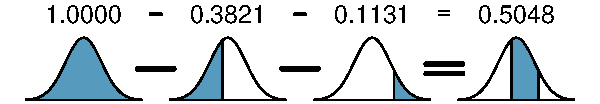
\includegraphics[width=60mm]{ch_inference_for_props/figures/p-hat_from_53_and_59_computation/p-hat_from_53_and_59_computation}
%\end{center}
\end{example}

\begin{exercise}
In Example~\ref{smallerSampleWhatHappensToPropErrorExercise}
we discussed how a smaller sample would tend
to produce a less reliable estimate. Explain how this intuition
is reflected in the formula for
$SE_{\hat{p}} = \sqrt{\frac{p (1 - p)}{n}}$.\footnote{Since the
sample size $n$ is in the denominator of the fraction (on the
bottom of the fraction), a bigger sample size means the entire
expression when calculated will tend to be smaller. That is,
a larger sample size would correspond to a smaller standard error.}
\end{exercise}

%In Example~\ref{sampling_10k_prop_56p}, we applied a general
%principle called the \term{Central Limit Theorem}
%\hiddenterm{Central Limit Theorem!proportions} when
%we used the normal distribution as an approximation.


\subsection{Applying the Central Limit Theorem to a real-world setting}

Think back to the 2018 poll where
$\hat{p} = \pewsolarpollprop{}$ of American adults favored
expanding solar energy. We might wonder: does the sample
proportion from the poll approximately follow a normal
distribution?
We check the conditions from the Central Limit Theorem:
\begin{description}
\item[Independence.] The poll is a simple random sample of
    American adults, which means that the observations are
    independent.
\item[Success-failure condition.] To check this condition,
    we need the population proportion, $p$, to check if both
    $np$ and $n(1-p)$ are greater than 10. However, we do not
    know the value of $p$; that's exactly why the pollsters
    took a sample! In cases like these, we often use $\hat{p}$
    as our next best way to check the success-failure condition:
    \begin{align*}
    n\hat{p} &= \pewsolarpollsize{} \times \pewsolarpollprop{}
        = \pewsolarpollcount{}
    &n (1 - \hat{p}) &= \pewsolarpollsize{} \times (1 - \pewsolarpollprop{})
        = \pewsolarpollcountcomplement{}
    \end{align*}
    While we cannot check the condition with $p$,
    $\hat{p}$ acts as a reasonable substitute, and we are comfortably
    above the minimums of 10.
\end{description}

This \term{substitution approximation} of using $\hat{p}$ in
place of $p$ will also be useful when computing the standard error
of the sample proportion in many situations:
\begin{align*}
SE_{\hat{p}}
    = \sqrt{\frac{p (1 - p)}{n}}
    \approx \sqrt{\frac{\hat{p} (1 - \hat{p})}{n}}
    \approx \sqrt{\frac{\pewsolarpollprop{}
        (1 - \pewsolarpollprop{})}{\pewsolarpollsize{}}}
    = \pewsolarpollse{}
\end{align*}
This substitution approximation technique is useful in many
situations.
%\footnote{There are additional methods
%for proportions that perform some correction for the substitution
%approximation. However, we leave those proportion methods for
%a future course.}




%__________________
\section[Confidence interval for a sample proportion]{Confidence
    intervals for a sample\\proportion} % \sectionvideohref{youtube-FUaXoKdCre4&list=PLkIselvEzpM7Pjo94m1e7J5jkIZkbQAl4}~\sectionslideshref{gdoc_os3_slides_4-2}}
\label{confidenceIntervals}

\index{confidence interval|(}

The sample proportion $\hat{p}$ provides a single plausible value
for the population proportion $p$. However, the sample proportion
isn't perfect and will have some \emph{standard error}
associated with it. Instead of supplying just this point estimate
of the population proportion, a next logical step would be
to provide a plausible \emph{range of values}.

\subsection{Capturing the population parameter}

A plausible range of values for the population parameter
is called a \term{confidence interval}.

Using only a point estimate is like fishing in a murky
lake with a spear, and using a confidence interval is
like fishing with a net. We can throw a spear where we
saw a fish, but we will probably miss. On the other hand,
if we toss a net in that area, we have a good chance of
catching the fish.

If we report a point estimate $\hat{p}$, we probably
will not hit the exact population proportion. On the
other hand, if we report a range of plausible values
-- a confidence interval -- we have a good shot at
capturing the parameter. 

\begin{exercise}
If we want to be very certain we capture the population
proportion in an interval, should we use a wider interval
or a smaller interval?\footnote{If we want to be more
certain we will capture the fish, we might use a
wider net. Likewise, we use a wider confidence interval
if we want to be more certain that we capture the
parameter.}
\end{exercise}

\subsection{An approximate 95\% confidence interval}

Our sample proportion $\hat{p}$ is the most plausible
value of the population proportion, so it makes sense
to build a confidence interval around this point estimate.
The \hiddenterm{standard error} provides a guide for how
large we should make the confidence interval.

The standard error represents the standard deviation
of with the point estimate, and when the Central
Limit Theorem conditions are satisfied, we also know
that the point estimate closely follows a normal
distribution. In a normal distribution, about 95\% of
the data is within 2 standard deviations of the mean.
Using this principle, we can construct a confidence
interval that extends 2 standard errors from the sample
proportion to be \term{95\% confident}\index{confident|textbf}
that the interval captures the population proportion:
\begin{align*}
\text{point estimate}\ &\pm\ 2\times SE \\
\hat{p}\ &\pm\ 2\times SE_{\hat{p}}
%\label{95PercentConfidenceIntervalFormula}
\end{align*}
But what does ``95\% confident'' mean? Suppose we took
many samples and built a 95\% confidence interval from
each sample. Then about 95\% of those intervals would
contain the parameter, $p$.
Figure~\ref{95PercentConfidenceInterval} shows this
process with 25 samples from the simulation in
Section~\ref{simulationForUnderstandingVariabilitySection},
where 24 of the resulting confidence intervals contain
the simulation's population proportion of
$p = \pewsolarpollprop{}$, and one interval does not.

\begin{figure}
   \centering
   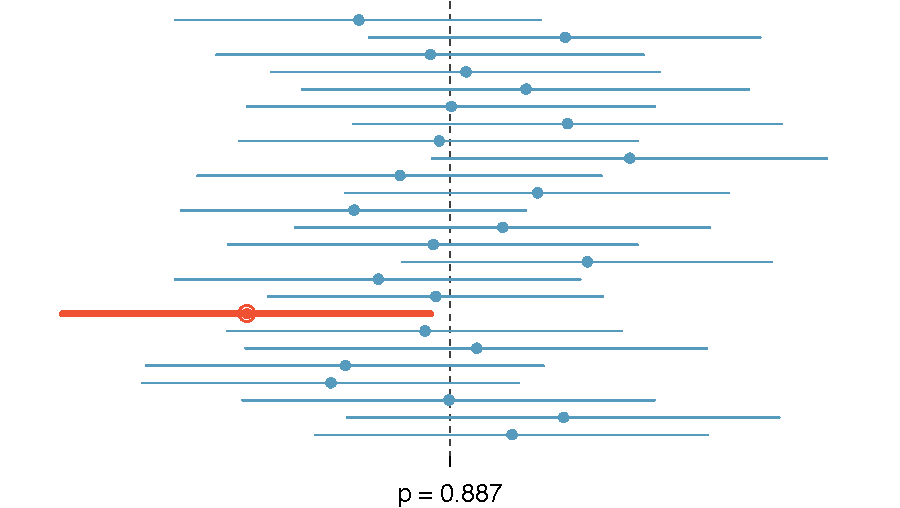
\includegraphics[width=0.75\textwidth]{ch_inference_for_props/figures/95PercentConfidenceInterval/95PercentConfidenceInterval}
   \caption{Twenty-five point estimates and confidence
       intervals from the simulations in
       Section~\ref{simulationForUnderstandingVariabilitySection}.
       For~each sample, a 95\% confidence interval was
       constructed and shown relative to the population
       proportion $p = \pewsolarpollprop{}$. Only~1 of these~25
       intervals did not capture the true population
       proportion.}
   \label{95PercentConfidenceInterval}
\end{figure}

\begin{example}{In Figure~\ref{95PercentConfidenceInterval},
one interval does not contain $p = \pewsolarpollprop{}$.
Does this imply that the population proportion cannot be
$p = \pewsolarpollprop{}$?}
Just as some observations occur more than 2 standard deviations
from the mean, some point estimates will be more than
2 standard errors from the parameter of interest.
A confidence interval only provides a plausible range
of values. While we might say other values are implausible
based on the data, this does not mean they are impossible.
\end{example}

While about 95\% of the data is within 2 standard deviations
in a normal distribution, it would be more precise to use
a value of 1.96 standard deviations. This more precise value
is what is used to construct standard confidence intervals.

\begin{termBox}{\tBoxTitle{95\% confidence interval for
    a parameter}
  When a point estimate qualifies for the Central Limit
  Theorem and closely follows a normal distribution,
  we can construct a 95\% confidence interval as
  \begin{align*}
  \text{point estimate} &\pm 1.96 \times SE
  \end{align*}}
\end{termBox}

\begin{example}{In Section~\ref{pointEstimates} we learned about
    a poll where \pewsolarpollpercent{}\% of a random sample of
    \pewsolarpollsize{} American adults
    supported expanding the role of solar power. Compute and
    interpret a 95\% confidence interval for the population
    proportion.} \label{95p_ci_for_pew_solar_support}
  We earlier confirmed that $\hat{p}$ follows a normal
  distribution and has a standard error is
  $SE_{\hat{p}} = \pewsolarpollse{}$.
  To compute the 95\% confidence interval, we plug the
  point estimate $\hat{p} = \pewsolarpollprop{}$ and
  standard error into the 95\% confidence interval formula:
  \begin{align*}
  \hat{p} \pm 1.96 \times SE_{\hat{p}}
  \quad\to\quad
  \pewsolarpollprop{} \pm 1.96 \times \pewsolarpollse{}
  \quad\to\quad
  (0.8674, 0.9066)
  \end{align*}
  We are 95\% confident that the actual proportion of
  American adults who support expanding solar power is
  between 86.74\% and 90.66\%.
\end{example}


\subsection{Changing the confidence level}
\label{changingTheConfidenceLevelSection}

\index{confidence interval!confidence level|(}

Suppose we want to consider confidence intervals where the confidence
level is somewhat higher than 95\%; perhaps we would like a confidence
level of 99\%. Think back to the analogy about trying to catch a fish:
if~we want to be more sure that we will catch the fish, we should use
a wider net. To create a 99\% confidence level, we must also widen our
95\% interval. On the other hand, if we want an interval with lower
confidence, such as 90\%, we could make our original 95\% interval
slightly slimmer.

The 95\% confidence interval structure provides guidance in how to
make intervals with new confidence levels. The general 95\% confidence
interval for a point estimate that follows the normal distribution is
normal distribution:
\begin{eqnarray}
\text{point estimate}\ \pm\ 1.96\times SE
\end{eqnarray}
There are three components to this interval: the point estimate $\hat{p}$,
``1.96'', and the standard error. The choice of $1.96\times SE$ was
based on capturing 95\% of the data since the estimate is within 1.96
standard errors of the parameter about 95\% of the time.
The choice of 1.96 corresponds to a 95\% confidence level. 

\begin{exercise} \label{leadInForMakingA99PercentCIExercise}
If $X$ is a normally distributed random variable, how often will $X$
be within 2.58 standard deviations of the mean?\footnote{This is
equivalent to asking how often the Z-score will be larger than -2.58
but less than 2.58. (For a picture, see Figure~\ref{choosingZForCI}.)
To determine this probability, we can use statistical software,
a calculator, or a table to look up -2.58 and 2.58 for the normal
distribution: 0.0049 and 0.9951. Thus, there is a
$0.9951-0.0049 \approx 0.99$ probability that an unobserved random
variable $X$ will be within 2.58 standard deviations of $\mu$.}
\end{exercise}

To create a 99\% confidence interval, change 1.96 in the 95\%
confidence interval formula to be $2.58$. Guided Practice~\ref{leadInForMakingA99PercentCIExercise} highlights
that 99\% of the time a normal random variable will be within
2.58 standard deviations of the mean. This approach -- using
the Z-scores in the normal model to compute confidence levels -- is
appropriate when $\hat{p}$ is associated with a normal distribution
with mean $p$ and standard error $SE_{\hat{p}}$. Thus, the formula
for a 99\% confidence interval for $\hat{p}$ is
\begin{eqnarray}
\hat{p}\ \pm\ 2.58\times SE_{\hat{p}}
%\label{99PercCIForMean}
\label{99PercCIForProp}
\end{eqnarray}

\begin{figure}
  \centering
  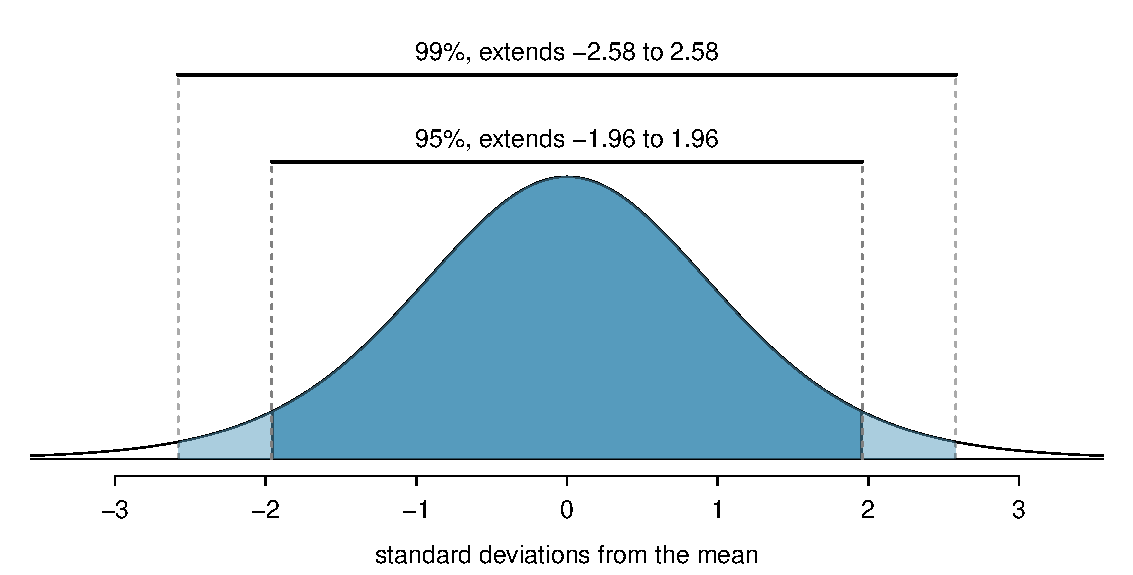
\includegraphics[width=\textwidth]{ch_inference_for_props/figures/choosingZForCI/choosingZForCI}
  \caption{The area between -$z^{\star}$ and $z^{\star}$ increases as
      $z^{\star}$ becomes larger. If the confidence level is 99\%,
      we choose $z^{\star}$ such that 99\% of the normal curve is
      between -$z^{\star}$ and $z^{\star}$, which corresponds to 0.5\%
      in the lower tail and 0.5\% in the upper tail: $z^{\star}=2.58$.}
\label{choosingZForCI}
\index{confidence interval!confidence level|)}
\end{figure}

The normal approximation is crucial to the precision of these
confidence intervals. For the context of sample proportions, the
normal distribution is reasonable to use whenever the sample
observations are independent and the success-failure condition
holds ($np$ and $n(1-p)$ are both at least 10).
For some other point estimates, the normal model is not a good fit.
In these cases, we'll use alternative distributions that better
represent the sampling distribution.

\begin{tipBox}{\tipBoxTitle[]{How to verify sample observations
    are independent}
  Subjects in an experiment are considered independent if they undergo
      random assignment to the treatment groups. \\[2mm]
  If the observations are from a simple random sample and consist
      of fewer than 10\% of the population, then they are independent.
      Even if the sample is bigger than 10\%, assuming independence
      will lead to more conservative results. \\[2mm]
  If a sample is from a seemingly random process,
      e.g. an occasional error on an assembly line,
      checking independence is more difficult. In~this case,
      use your best judgement.}
\end{tipBox}

\begin{termBox}{\tBoxTitle{Confidence interval for $p$ using any confidence level}
  If $\hat{p}$ approximately follows the normal model with
  standard error $SE_{hat{p}}$, then a confidence interval
  for the population parameter is
  \begin{eqnarray*}
  \hat{p}\ \pm\ z^{\star} SE_{\hat{p}}
  \end{eqnarray*}
  where $z^{\star}$ corresponds to the confidence level selected.}
\end{termBox}

Figure~\ref{choosingZForCI} provides a picture of how to identify
$z^{\star}$ based on a confidence level. We~select $z^{\star}$
so that the area between -$z^{\star}$ and $z^{\star}$ in the normal
model corresponds to the confidence level. 

\begin{termBox}{\tBoxTitle{Margin of error}
\label{marginOfErrorTermBox}
In a confidence interval, $z^{\star}\times SE$ is called the
\term{margin of error}.}
\end{termBox}

\begin{example}{Use the data in
    Example~\ref{95p_ci_for_pew_solar_support} to
    create a 90\% confidence interval for the proportion of American
    adults that support expanding solar power students.}
  We first find $z^{\star}$ such that 90\% of the distribution falls
  between -$z^{\star}$ and $z^{\star}$ in the standard normal model,
  $N(\mu=0, \sigma=1)$. We can do this using a graphing calculator,
  statistical software, or a probability table by looking for a lower
  tail of 5\% (the other 5\% is in the upper tail): $z^{\star}=1.65$.
  The 90\% confidence interval can then be computed as
  $\hat{p}\ \pm\ 1.65\times SE_{\hat{p}} \to (0.8705, 0.9035)$.
  (We had already verified conditions for normality and the standard error.)
  That is, we are 90\% confident that 87.1\% to 90.4\% of American
  adults support the expansion of solar power in 2018.
\end{example}



\subsection{Two case studies}

\index{data!Ebola poll|(}

\newcommand{\wsjebolapollsize}{1042}
\newcommand{\wsjebolapollsizecomma}{1,042}
\newcommand{\wsjebolapollprop}{0.82}
\newcommand{\wsjebolapollpropcomplement}{0.18}
\newcommand{\wsjebolapollpercent}{82}
\newcommand{\wsjebolapollpercentcomplement}{18}
\newcommand{\wsjebolapollcount}{854}
\newcommand{\wsjebolapollcountcomplement}{188}
\newcommand{\wsjebolapollse}{0.012}


In New York City on October 23rd, 2014, a doctor who had recently been
treating Ebola patients in Guinea went to the hospital with a slight fever
and was subsequently diagnosed with Ebola. Soon thereafter,
an NBC~4 New York/The Wall Street Journal/Marist Poll found that
\wsjebolapollpercent{}\% of New Yorkers favored a ``mandatory 21-day
quarantine for anyone who has come in contact with an Ebola
patient''.\footnote{\oiRedirect{textbook-maristpoll_ebola_201410}{Poll
ID NY141026 on maristpoll.marist.edu}.} This poll included responses
of \wsjebolapollsizecomma{} New York adults between October 26th and~28th,
2014. We may want a confidence interval for the proportion of New York
adults who favored a mandatory quarantine of anyone who had been in
contact with an Ebola patient.

\begin{example}{What is the point estimate in this case,
    and is it reasonable to
    use the normal distribution to model that point estimate?}
  The point estimate, based on a sample of size $n = \wsjebolapollsize{}$,
  is $\hat{p} = \wsjebolapollprop{}$. To check whether $\hat{p}$ can be reasonably
  modeled using the normal distribution, we check independence
  (the poll is based on a simple random sample) and the
  success-failure condition
  ($\wsjebolapollsize{} \times \hat{p} \approx \wsjebolapollcount{}$
  and $\wsjebolapollsize{} \times (1 - \hat{p})
      \approx \wsjebolapollcountcomplement{}$,
  both easily greater than~10). With the conditions met, we are assured
  that the sampling distribution of $\hat{p}$ can be modeled using
  a normal distribution.
\end{example}

\begin{example}{Estimate the standard error of
    $\hat{p} = \wsjebolapollprop{}$ from the Ebola survey.}
  We'll use the substitution approximation of
  $p \approx \hat{p} = \wsjebolapollprop{}$ to compute the standard error:
  \footnote{$SE = \sqrt{\frac{p(1-p)}{n}}
    \approx \sqrt{\frac{\wsjebolapollprop{}
        (1 - \wsjebolapollprop{})}{\wsjebolapollsize{}}}
    = \wsjebolapollse{}$.}
\end{example}

\begin{example}{Construct a 95\% confidence interval for $p$,
    the proportion of New York adults who supported a quarantine
    for anyone who has come into contact with an Ebola patient.}
  Using the standard error $SE = 0.012$ from
  Example~\ref{seOfPropOfAmericansJobApprovalOfSupremeCourt},
  the point estimate \wsjebolapollprop{}, and $z^{\star} = 1.96$
  for a 95\% confidence interval, the confidence interval is
  \begin{eqnarray*}
  \text{point estimate} \ \pm\ z^{\star}SE
    \quad\to\quad \wsjebolapollprop{} \ \pm\ 1.96\times \wsjebolapollse{}
    \quad\to\quad (0.796, 0.844)
  \end{eqnarray*}
  We are 95\% confident that the proportion of New York adults
  in October 2014 who supported a quarantine for anyone who had come
  into contact with an Ebola patient was between 0.796 and 0.844.
\index{data!Ebola poll|)}
\end{example}

\begin{exercise}
Do you think the confidence interval is still valid for the opinions
of New Yorkers today?\footnote{No. The poll was taken at a
time where there was a huge public safety concern. Now that people
have had some time to step back, they may have changed their opinions.
We would need to run a new poll if we wanted to get an estimate of the
current proportion of New York adults who would support such a
quarantine period.}
\end{exercise}

\index{data!wind turbine survey|(}

\newcommand{\pewwindpollsize}{\pewsolarpollsize}
\newcommand{\pewwindpollprop}{0.848}
\newcommand{\pewwindpollpropcomplement}{0.152}
\newcommand{\pewwindpollpercent}{84.8}
\newcommand{\pewwindpollpercentcomplement}{15.2}
\newcommand{\pewwindpollcount}{848}
\newcommand{\pewwindpollcountcomplement}{152}
\newcommand{\pewwindpollse}{0.0114}

In the same survey asking about Americans' support of expanding
solar energy usage, Pew Research asked the same question about
wind turbines and found support from \pewwindpollpercent{}\%
of respondents.

\begin{exercise}\label{pew_wind_turbine_support_normal_dist_gp}
Is the normal approximation reasonable in this case?\footnote{We
check independence, which is okay since this survey was a simple
random sample, and also the success-failure condition
($\pewwindpollsize{} \times \pewwindpollprop{} = \pewwindpollcount{}$
and $\pewwindpollsize{} \times \pewwindpollpropcomplement{}
    = \pewwindpollcountcomplement$ are both at least 10).
Since both are satisfied, $\hat{p} = \pewwindpollprop{}$ can be
modeled using the normal distribution.}
\end{exercise}

\begin{exercise}
Using the Pew Research survey where $n = \pewwindpollsize{}$ and
$\hat{p} = \pewwindpollprop{}$, create a 99\% confidence interval
for the level of American support for expanding the use of wind
turbines for power
generation?\footnote{Guided
Practice~\ref{pew_wind_turbine_support_normal_dist_gp}
confirmed that that $\hat{p}$ closely follows a normal distribution,
so we can use the confidence interval formula:
\begin{align*}
\text{point estimate} \pm z^{\star} SE
\end{align*}
In this case, the point estimate is $\hat{p} = \pewwindpollprop{}$.
For a 99\% confidence interval, $z^{\star} = 2.58$. Computing the
standard error:
$SE_{\hat{p}}
  = \sqrt{\frac{\pewwindpollprop{}(1 - \pewwindpollprop{})}
      {\pewwindpollsize{}}}
  = \pewwindpollse{}$.
Finally, we compute the interval as
$\pewwindpollprop{} \pm 2.58 \times \pewwindpollse{} \to (0.8186, 0.8774)$.
It is also \emph{always} important to provide an interpretation for
the interval: we are 99\% confident the proportion of
Americans adults that support expanding the use of wind
turbines is between 81.9\% and 87.7\% in 2018.}
\end{exercise}




\subsection{Interpreting confidence intervals}
\label{interpretingCIs}

\index{confidence interval!interpretation|(}

In each of the examples, we described the confidence
intervals by putting them into the context of the data and also
using somewhat formal language:
\begin{description}
  \item[Solar.] We are 90\% confident that 87.1\% to 90.4\% of
      American adults support the expansion of solar power in 2018.
  \item[Ebola.] We are 95\% confident that the proportion
      of New York adults in October 2014 who supported a quarantine
      for anyone who had come into contact with an Ebola patient was
      between 0.796 and 0.844.
  \item[Wind Turbine.] We are 99\% confident the proportion of
      Americans adults that support expanding the use of wind
      turbines is between 81.9\% and 87.7\% in 2018.
\end{description}
First, notice that the statements are always about the population
parameter, which is American adults in this case, \emph{not} only
the adults included in the sample.

We also avoided another common mistake:
\emph{incorrect} language might try to describe the confidence interval
as capturing the population parameter with a certain probability.
Making a probability interpretation is a common error:
while it might be useful to think of it as a probability,
the confidence level only quantifies how plausible
it is that the parameter is in the interval.

Another important consideration of confidence intervals is that they
\emph{only try to capture the population parameter}. A confidence
interval says nothing about the confidence of capturing individual
observations, a proportion of the observations, or about capturing
point estimates. Confidence intervals only attempt to capture
population parameters.

\index{data!wind turbine survey|)}
\index{data!solar survey|)}
\index{confidence interval!interpretation|)}
\index{confidence interval|)}




\section{Hypothesis testing for the 1-proportion context}
\label{hypothesis_testing_one_prop}







%__________________
\subsection{Hypothesis testing for a proportion}
\label{hypothesisTesting}
%\section[Hypothesis testing]{Hypothesis testing \sectionvideohref{youtube-NVbPE1_Cbx8&list=PLkIselvEzpM7Pjo94m1e7J5jkIZkbQAl4}~\sectionslideshref{gdoc_os3_slides_4-3}}

\index{hypothesis testing|(}

Are students lifting weights or performing other strength training exercises more or less often than they have in the past? We'll compare data from students from the 2011 YRBSS survey to our sample of 100 students from the 2013 YRBSS survey.

We'll also consider sleep behavior. A recent study found that college students average about 7~hours of sleep per night.\footnote{\oiRedirect{textbook-theloquitur_1161}{\emph{Poll shows college students get least amount of sleep}. theloquitur.com/?p=1161}} However, researchers at a rural college are interested in showing that their students sleep longer than seven hours on average. We investigate this topic in Section~\ref{pValue}.

\subsection{Hypothesis testing framework}

Students from the 2011 YRBSS lifted weights (or performed other strength training exercises) 3.09~days per week on average. We want to determine if the \data{yrbss\_samp} data set provides strong evidence that YRBSS students selected in 2013 are lifting more or less than the 2011 YRBSS students, versus the other possibility that there has been no change.\footnote{While we could answer this question by examining the entire YRBSS data set from 2013 (\data{yrbss}), we only consider the sample data (\data{yrbss\_samp}), which is more realistic since we rarely have access to population data.} We simplify these three options into two competing \termsub{hypotheses}{hypothesis}:
\begin{itemize}
\setlength{\itemsep}{0mm}
\item[$H_0$:] The average days per week that YRBSS students lifted weights was the same for 2011 and~2013.
\item[$H_A$:] The average days per week that YRBSS students lifted weights was \emph{different} for 2013 than~in~2011.
\end{itemize}
We call $H_0$\marginpar[\raggedright\vspace{6mm}

$H_0$\\\footnotesize null hypothesis\vspace{3mm}\\\normalsize $H_A$\\\footnotesize alternative\\ hypothesis]{\raggedright\vspace{6mm}

$H_0$\\\footnotesize null hypothesis\vspace{3mm}\\\normalsize $H_A$\\\footnotesize alternative\\ hypothesis} the null hypothesis and $H_A$ the alternative hypothesis.

\begin{termBox}{\tBoxTitle{Null and alternative hypotheses}
{\small The \term{null hypothesis ($H_0$)} often represents either a skeptical perspective or a claim to be tested. The \term{alternative hypothesis ($H_A$)} represents an alternative claim under consideration and is often represented by a range of possible parameter values.}}
\end{termBox}

The null hypothesis often represents a skeptical position or a perspective of no difference. The alternative hypothesis often represents a new perspective, such as the possibility that there has been a change. 

\begin{tipBox}{\tipBoxTitle{Hypothesis testing framework}
The skeptic will not reject the null hypothesis ($H_0$), unless the evidence in favor of the alternative hypothesis ($H_A$) is so strong that she rejects $H_0$ in favor of $H_A$.}
\end{tipBox}

The hypothesis testing framework is a very general tool, and we often use it without a second thought. If a person makes a somewhat unbelievable claim, we are initially skeptical. However, if there is sufficient evidence that supports the claim, we set aside our skepticism and reject the null hypothesis in favor of the alternative. The hallmarks of hypothesis testing are also found in the US court system. 

\begin{exercise} \label{hypTestCourtExample}
A US court considers two possible claims about a defendant: she is either innocent or guilty. If we set these claims up in a hypothesis framework, which would be the null hypothesis and which the alternative?\footnote{The jury considers whether the evidence is so convincing (strong) that there is no reasonable doubt regarding the person's guilt; in such a case, the jury rejects innocence (the null hypothesis) and concludes the defendant is guilty (alternative hypothesis).}
\end{exercise}

Jurors examine the evidence to see whether it convincingly shows a defendant is guilty. Even if the jurors leave unconvinced of guilt beyond a reasonable doubt, this does not mean they believe the defendant is innocent. This is also the case with hypothesis testing: \emph{even if we fail to reject the null hypothesis, we typically do not accept the null hypothesis as true}. Failing to find strong evidence for the alternative hypothesis is not equivalent to accepting the null hypothesis.

In the example with the YRBSS, the null hypothesis represents no difference in the average days per week of weight lifting in 2011 and 2013. The alternative hypothesis represents something new or more interesting: there was a difference, either an increase or a decrease. These hypotheses can be described in mathematical notation using $\mu_{13}$ as the average days of weight lifting for 2013:
\begin{itemize}
\setlength{\itemsep}{0mm}
\item[$H_0$:] $\mu_{13} = 3.09$
\item[$H_A$:] $\mu_{13} \neq 3.09$
\end{itemize}
where 3.09 is the average number of days per week that students from the 2011 YRBSS lifted weights. Using the mathematical notation, the hypotheses can more easily be evaluated using statistical tools. We call 3.09 the \term{null value} since it represents the value of the parameter if the null hypothesis is true.


\subsection{Testing hypotheses using confidence intervals}
\label{utilizingOurCI}

We will use the \data{yrbss\_samp} data set to evaluate the hypothesis test, and we start by comparing the 2013 point estimate of the number of days per week that students lifted weights: $\bar{x}_{13} = 2.78$~days. This estimate suggests that students from the 2013 YRBSS were lifting weights less than students in the 2011 YRBSS. However, to evaluate whether this provides strong evidence that there has been a change, we must consider the uncertainty associated with $\bar{x}_{13}$.

We learned in Section~\ref{variabilityInEstimates} that there is fluctuation from one sample to another, and it is unlikely that the sample mean will be exactly equal to the parameter; we should not expect $\bar{x}_{13}$ to exactly equal $\mu_{13}$. Given that $\bar{x}_{13} = 2.78$, it might still be possible that the average of all students from the 2013 YRBSS survey is the same as the average from the 2011 YRBSS survey. The difference between $\bar{x}_{13}$ and 3.09 could be due to \emph{sampling variation}, i.e. the variability associated with the point estimate when we take a random sample.

In Section~\ref{confidenceIntervals}, confidence intervals were introduced as a way to find a range of plausible values for the population mean.

\begin{example}{In the sample of 100 students from the 2013 YRBSS survey, the average number of days per week that students lifted weights was 2.78~days with a standard deviation of 2.56 days (coincidentally the same as days active). Compute a 95\% confidence interval for the average for all students from the 2013 YRBSS survey. You can assume the conditions for the normal model are met.}
The general formula for the confidence interval based on the normal distribution is
\begin{align*}
\bar{x} \pm z^{\star} SE_{\bar{x}}
\end{align*}
We are given $\bar{x}_{13} = 2.78$, we use $z^{\star} = 1.96$ for a 95\% confidence level, and we can compute the standard error using the standard deviation divided by the square root of the sample size:
\begin{align*}
SE_{\bar{x}} = \frac{s_{13}}{\sqrt{n}} = \frac{2.56}{\sqrt{100}} = 0.256
\end{align*}
Entering the sample mean, $z^{\star}$, and the standard error into the confidence interval formula results in (2.27, 3.29). We are 95\% confident that the average number of days per week that all students from the 2013 YRBSS lifted weights was between 2.27~and 3.29~days.
\end{example}

Because the average of all students from the 2011 YRBSS survey is 3.09, which falls within the range of plausible values from the confidence interval, we cannot say the null hypothesis is implausible. That is, we fail to reject the null hypothesis, $H_0$.

\begin{tipBox}{\tipBoxTitle{Double negatives can sometimes be used in statistics}
In many statistical explanations, we use double negatives. For instance, we might say that the null hypothesis is \emph{not implausible} or we \emph{failed to reject} the null hypothesis. Double negatives are used to communicate that while we are not rejecting a position, we are also not saying it is correct.}
\end{tipBox}

\begin{exercise} \label{htForHousingExpenseForCommunityCollege650}
Colleges frequently provide estimates of student expenses such as housing. A consultant hired by a community college claimed that the average student housing expense was \$650 per month. What are the null and alternative hypotheses to test whether this claim is accurate?\footnote{$H_0$: The average cost is \$650 per month, $\mu = \$650$.

\hspace{3.4mm}$H_A$: The average cost is different than \$650 per month, $\mu \neq \$650$.}
\end{exercise}

\begin{exercise} \label{normalDistCondForHousingExpenseForCommunityCollege650}
The community college decides to collect data to evaluate the \$650 per month claim. They take a random sample of 175 students at their school and obtain the data represented in Figure~\ref{communityCollegeClaimedHousingExpenseDistribution}. Can we apply the normal model to the sample mean?\footnote{Applying the normal model requires that certain conditions are met. Because the data are a simple random sample and the sample (presumably) represents no more than 10\% of all students at the college, the observations are independent. The sample size is also sufficiently large ($n = 175$) and the data exhibit strong skew. While the data are strongly skewed, the sample is sufficiently large that this is acceptable, and the normal model may be applied to the sample mean.}

\begin{figure}
\centering
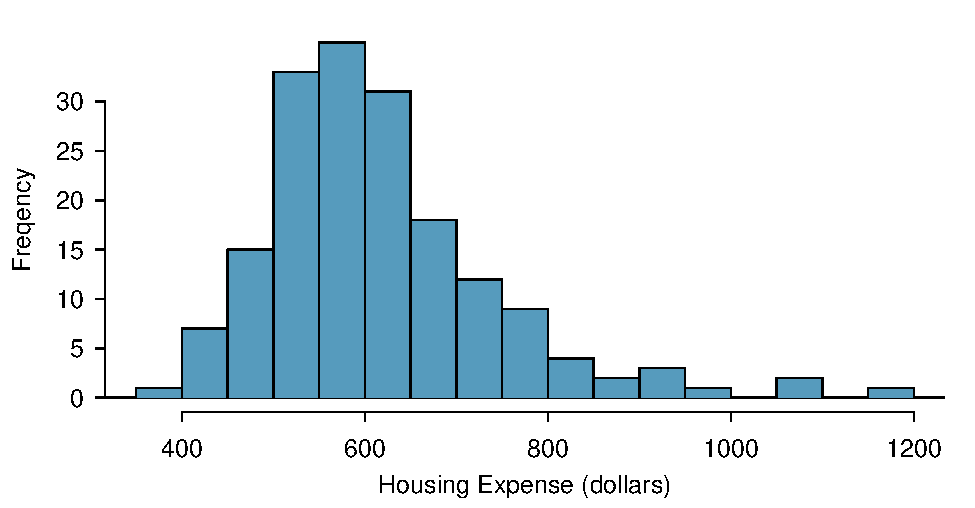
\includegraphics[width=0.9\textwidth]{ch_inference_for_props/figures/communityCollegeClaimedHousingExpenseDistribution/communityCollegeClaimedHousingExpenseDistribution}
\caption{Sample distribution of student housing expense. These data are strongly skewed\index{skew!example: strong}, which we can see by the long right tail with a few notable outliers.}
\label{communityCollegeClaimedHousingExpenseDistribution}
\end{figure}
\end{exercise}

\begin{tipBox}{\tipBoxTitle[]{Evaluating the skew condition is challenging}
Don't despair if checking the skew condition is difficult or confusing. You aren't alone -- nearly all students get frustrated when checking skew. Properly assessing skew takes practice, and you won't be a pro, even at the end of this book. \\[2mm]
But this doesn't mean you should give up. Checking skew and the other conditions is extremely important for a responsible data analysis. However, rest assured that evaluating skew isn't something you need to be a master of by the end of the book, though by that time you should be able to properly assess clear cut cases.}
\end{tipBox}

\textC{\newpage}

\begin{example}{The sample mean for student housing is \$616.91 and the sample standard deviation is \$128.65. Construct a 95\% confidence interval for the population mean and evaluate the hypotheses of Guided Practice~\ref{htForHousingExpenseForCommunityCollege650}.}
The standard error associated with the mean may be estimated using the sample standard deviation divided by the square root of the sample size. Recall that $n = 175$ students were sampled.
\begin{align*}
SE = \frac{s}{\sqrt{n}} = \frac{128.65}{\sqrt{175}} = 9.73
\end{align*}
You showed in Guided Practice~\ref{normalDistCondForHousingExpenseForCommunityCollege650} that the normal model may be applied to the sample mean. This ensures a 95\% confidence interval may be accurately constructed:
$$\bar{x}\ \pm\ z^{\star} SE \quad\to\quad 616.91\ \pm\ 1.96 \times 9.73 \quad \to \quad (597.84, 635.98) $$
Because the null value \$650 is not in the confidence interval, a true mean of \$650 is implausible and we reject the null hypothesis. The data provide statistically significant evidence that the actual average housing expense is less than \$650 per month.
\end{example}


\subsection{Decision errors}

\index{hypothesis testing!decision errors|(}

Hypothesis tests are not flawless, since we can make a wrong decision in statistical hypothesis tests based on the data. For example, in the court system innocent people are sometimes wrongly convicted and the guilty sometimes walk free. However, the difference is that in statistical hypothesis tests, we have the tools necessary to quantify how often we make such errors.

% Hypothesis tests are not flawless. Just think of the court system: innocent people are sometimes wrongly convicted and the guilty sometimes walk free. Similarly, we can make a wrong decision in statistical hypothesis tests. However, the difference is that we have the tools necessary to quantify how often we make such errors.

There are two competing hypotheses: the null and the alternative. In a hypothesis test, we make a statement about which one might be true, but we might choose incorrectly. There are four possible scenarios, which are summarized in Table~\ref{fourHTScenarios}.

\begin{table}[ht]
\centering
\begin{tabular}{l l c c}
& & \multicolumn{2}{c}{\textbf{Test conclusion}} \\
  \cline{3-4}
\vspace{-3.7mm} \\
& & do not reject $H_0$ &  reject $H_0$ in favor of $H_A$ \\
  \cline{2-4}
\vspace{-3.7mm} \\
& $H_0$ true & okay &  Type~1 Error \\
\raisebox{1.5ex}{\textbf{Truth}} & $H_A$ true & Type~2 Error & okay \\
  \cline{2-4}
\end{tabular}
\caption{Four different scenarios for hypothesis tests.}
\label{fourHTScenarios}
\end{table}

A \term{Type~1 Error} is rejecting the null hypothesis when $H_0$ is actually true. A \term{Type~2 Error} is failing to reject the null hypothesis when the alternative is actually true.

\begin{exercise} \label{whatAreTheErrorTypesInUSCourts}
In a US court, the defendant is either innocent ($H_0$) or  guilty ($H_A$). What does a Type~1 Error represent in this context? What does a Type~2 Error represent? Table~\ref{fourHTScenarios} may be useful.\footnote{If the court makes a Type~1 Error, this means the defendant is innocent ($H_0$ true) but wrongly convicted. A Type~2 Error means the court failed to reject $H_0$ (i.e. failed to convict the person) when she was in fact guilty ($H_A$ true).}
\end{exercise}

\begin{exercise} \label{howToReduceType1ErrorsInUSCourts}
How could we reduce the Type~1 Error rate in US courts? What influence would this have on the Type~2 Error rate?\footnote{To lower the Type~1 Error rate, we might raise our standard for conviction from ``beyond a reasonable doubt'' to ``beyond a conceivable doubt'' so fewer people would be wrongly convicted. However, this would also make it more difficult to convict the people who are actually guilty, so we would make more Type~2 Errors.}
\end{exercise}

\begin{exercise} \label{howToReduceType2ErrorsInUSCourts}
How could we reduce the Type~2 Error rate in US courts? What influence would this have on the Type~1 Error rate?\footnote{To lower the Type~2 Error rate, we want to convict more guilty people. We could lower the standards for conviction from ``beyond a reasonable doubt'' to ``beyond a little doubt''. Lowering the bar for guilt will also result in more wrongful convictions, raising the Type~1 Error rate.}
\end{exercise}

\index{hypothesis testing!decision errors|)}

Exercises~\ref{whatAreTheErrorTypesInUSCourts}-\ref{howToReduceType2ErrorsInUSCourts} provide an important lesson: if we reduce how often we make one type of error, we generally make more of the other type.

Hypothesis testing is built around rejecting or failing to reject the null hypothesis. That is, we do not reject $H_0$ unless we have strong evidence. But what precisely does \emph{strong evidence} mean? As a general rule of thumb, for those cases where the null hypothesis is actually true, we do not want to incorrectly reject $H_0$ more than 5\% of the time. This corresponds to a \term{significance level}\index{hypothesis testing!significance level} of 0.05. We often write the significance level using $\alpha$\marginpar[\raggedright\vspace{-4mm}

$\alpha$\\\footnotesize significance\\level of a\\hypothesis test]{\raggedright\vspace{-4mm}

$\alpha$\\\footnotesize significance\\level of a\\hypothesis test} (the Greek letter \emph{alpha}\index{Greek!alpha@alpha ($\alpha$)}): $\alpha = 0.05$. We discuss the appropriateness of different significance levels in Section~\ref{significanceLevel}.

If we use a 95\% confidence interval to evaluate a hypothesis test where the null hypothesis is true, we will make an error whenever the point estimate is at least 1.96 standard errors away from the population parameter. This happens about 5\% of the time (2.5\% in each tail). Similarly, using a 99\% confidence interval to evaluate a hypothesis is equivalent to a significance level of $\alpha = 0.01$.

A confidence interval is, in one sense, simplistic in the world of hypothesis tests. Consider the following two scenarios:
\begin{itemize}
\setlength{\itemsep}{0mm}
\item The null value (the parameter value under the null hypothesis) is in the 95\% confidence interval but just barely, so we would not reject $H_0$. However, we might like to somehow say, quantitatively, that it was a close decision.
\item The null value is very far outside of the interval, so we reject $H_0$. However, we want to communicate that, not only did we reject the null hypothesis, but it wasn't even close. Such a case is depicted in Figure~\ref{whyWeWantPValue}.
\end{itemize}
In Section~\ref{pValue}, we introduce a tool called the \emph{p-value} that will be helpful in these cases. The p-value method also extends to hypothesis tests where confidence intervals cannot be easily constructed or applied.

\begin{figure}[hht]
\centering
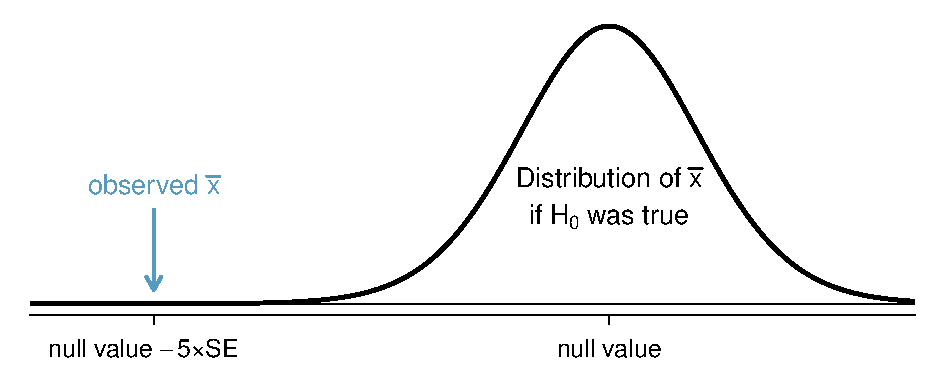
\includegraphics[width=0.75\textwidth]{ch_inference_for_props/figures/whyWeWantPValue/whyWeWantPValue}
\caption{It would be helpful to quantify the strength of the evidence against the null hypothesis. In this case, the evidence is extremely strong.}
\label{whyWeWantPValue}
\end{figure}



\subsection{Hypothesis testing for a proportion}

To apply the normal distribution framework in the context of a hypothesis test for a proportion, the independence and success-failure conditions must be satisfied. In a hypothesis test, the success-failure condition is checked using the null proportion: we verify $np_0$ and $n(1-p_0)$ are at least 10, where $p_0$ is the null value.

\index{data!nuclear arms reduction|(}

\begin{exercise}
Do a majority of American support nuclear arms reduction? Set up a one-sided hypothesis test to evaluate this question.\footnote{$H_0: p = 0.50$. $H_A: p > 0.50$.}
\end{exercise}

\begin{example}{A simple random sample of 1,028 US adults in March 2013 found that 56\% support nuclear arms reduction.\footnote{\oiRedirect{textbook-nuclear_arms_reduction_201303}{www.gallup.com/poll/161198/favor-russian-nuclear-arms-reductions.aspx}} Does this provide convincing evidence that a majority of Americans supported nuclear arms reduction at the 5\% significance level?} \label{NuclearArmsInferenceExample}
The poll was of a simple random sample that includes fewer than 10\% of US adults, meaning the observations are independent. In a one-proportion hypothesis test, the success-failure condition is checked using the null proportion, which is $p_0 = 0.5$ in this context: $n p_0 = n (1 - p_0) = 1028 \times 0.5 = 514 > 10$. With these conditions verified, the normal model may be applied to $\hat{p}$.

Next the standard error can be computed. The null value $p_0$ is used again here, because this is a hypothesis test for a single proportion.
\begin{align*}
SE = \sqrt{\frac{p_0 (1 - p_0)}{n}} = \sqrt{\frac{0.5 (1 - 0.5)}{1028}} = 0.016
\end{align*}
A picture of the normal model is shown in Figure~\ref{nuclearArmsReductionPValue} with the p-value represented by the shaded region. Based on the normal model, the test statistic can be computed as the Z-score of the point estimate:
\begin{align*}
Z = \frac{\text{point estimate} - \text{null value}}{SE} = \frac{0.56 - 0.50}{0.016} = 3.75
\end{align*}
The upper tail area, representing the p-value, is about 0.0001. Because the p-value is smaller than 0.05, we reject $H_0$. The poll provides convincing evidence that a majority of Americans supported nuclear arms reduction efforts in March 2013.
\end{example}

\begin{figure}[h]
\centering
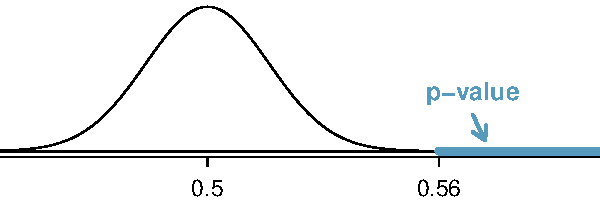
\includegraphics[width=0.48\textwidth]{ch_inference_for_props/figures/nuclearArmsReduction/nuclearArmsReductionPValue}
\caption{Sampling distribution for Example~\ref{NuclearArmsInferenceExample}.}
\label{nuclearArmsReductionPValue}
\end{figure}

\begin{termBox}{\tBoxTitle{Hypothesis test for a proportion}
Set up hypotheses and verify the conditions using the null value, $p_0$, to ensure $\hat{p}$ is nearly normal under $H_0$. If the conditions hold, construct the standard error, again using $p_0$, and show the p-value in a drawing. Lastly, compute the p-value and evaluate the hypotheses.}
\end{termBox}

\index{data!nuclear arms reduction|)}

\CalculatorVideos{confidence intervals and hypothesis tests for a single proportion}




















\section{Better understanding the Central Limit Theorem}


\subsection{Why do we have the $np \geq 10$ and
    $n(1-p) \geq 10$ rules?}

We've only looked at one situation so far: when the sample
proportion is $p = 0.56$ and the sample size is $n = 1000$.
What happens if we have a different proportion or sample size?

Let's start by considering different sample sizes.
Figure~\ref{sampling_X_prop_56p} shows the distribution of sample
proportions when the sample size is 5, 25, and 100. There are
two key takeaways:
\begin{itemize}
\item When the sample size is very small, the distribution has
very discrete properties: it doesn't look very smooth. However,
for larger sample sizes, the distribution looks smoother and
more like a normal distribution.
\item The bigger the sample size, the more often the estimate is
close to the population proportion $p = 0.56$. This is intuitive:
bigger samples will tend to produce more accurate estimates.
\end{itemize}

\begin{figure}
   \centering
   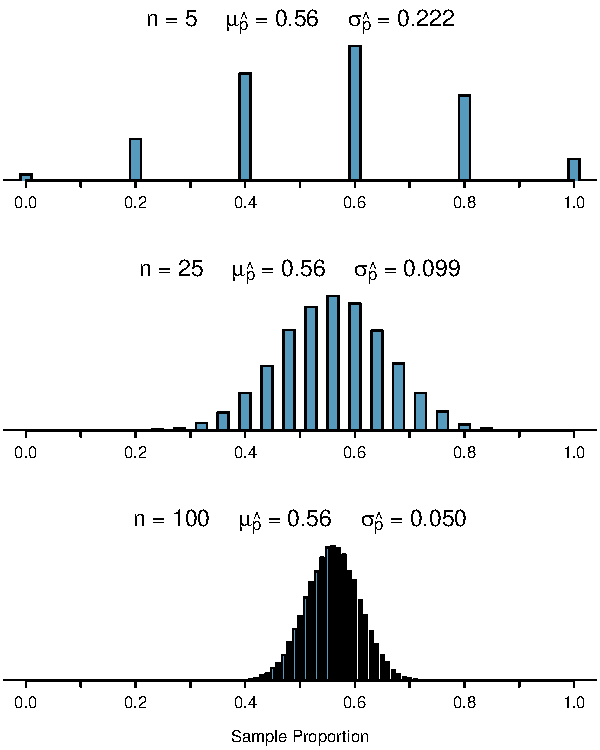
\includegraphics[width=0.67\textwidth]{ch_inference_for_props/figures/sampling_X_prop_56p/sampling_X_prop_56p}
   \caption{Simulations of $\hat{p}$ when the population
       proportion is $p = 0.56$ and for the following sample sizes:
       $n = 5$, $n = 25$, and $n = 100$. The theoretical
       mean~($\mu_{\hat{p}}$) and standard
       deviation~($SE_{\hat{p}}$) is also provided for each plot.}
   \label{sampling_X_prop_56p}
\end{figure}

%\begin{termBox}{\tBoxTitle{Law of Large Numbers for proportions}
%  \hiddenterm{Law of Large Numbers!proportions}
%  When the sample size is large, the sample proportion tends to be
%  a more reliable estimate of the population proportion.}
%\end{termBox}

Next let's consider what happens when we use different proportions.
For this exploration, let's use a sample size of $n = 100$ and
proportions of 0.03, 0.20, 0.50 0.80, and 0.97. The distributions
are shown in Figure~\ref{sampling_X_prop_56p}. Below are key
takeaways from these simulations:
\begin{itemize}
\item When the population proportion $p$ is close to 0 or 1, the
    distribution of sample proportions tends to be skewed. However,
    for proportions relatively far from   gets larger, the
    distribution becomes more symmetric
\item The estimates tend to be less variable when the proportion
    is near 0 or 1, as is shown by their lower variability listed
    in the table.
\end{itemize}

\begin{figure}
   \centering
   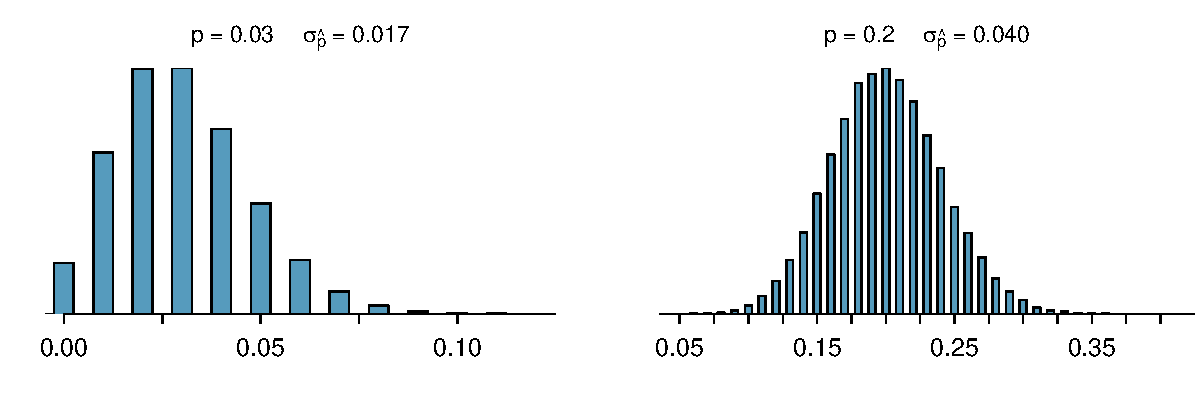
\includegraphics[width=\textwidth]{ch_inference_for_props/figures/sampling_100_prop_X/sampling_100_prop_X_12}
   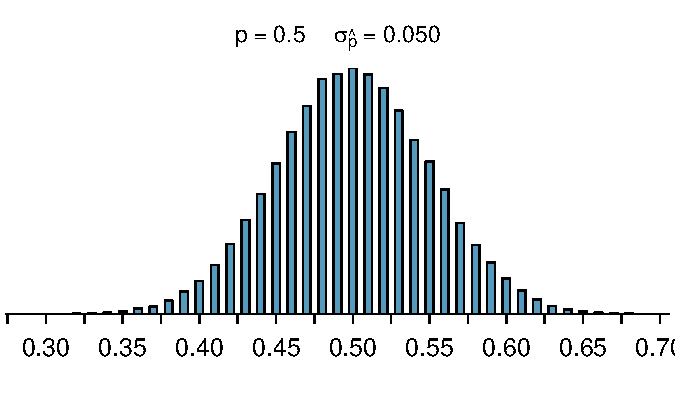
\includegraphics[width=0.55\textwidth]{ch_inference_for_props/figures/sampling_100_prop_X/sampling_100_prop_X_3}
   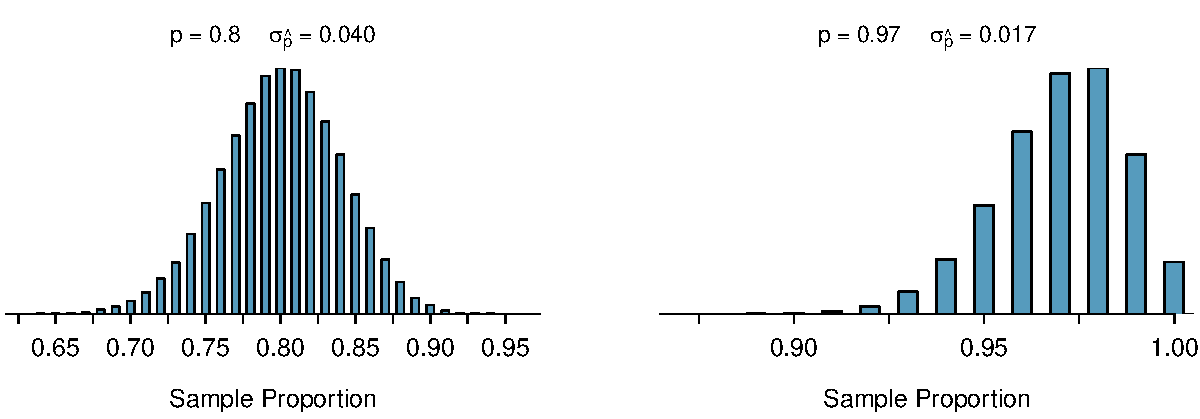
\includegraphics[width=\textwidth]{ch_inference_for_props/figures/sampling_100_prop_X/sampling_100_prop_X_45}
   \caption{Simulations of $\hat{p}$ for different population
       proportions when the sample size is $n = 100$. Each plot
       is centered at the population proportion $p$, and the
       theoretical standard deviation ($SE_{\hat{p}}$) is
       also provided for each plot.}
   \label{sampling_X_prop_56p}
\end{figure}

\Comment{Make sure the plots show $SE_{\hat{p}}$ rather than $\sigma_{\hat{p}}$.}


\subsection{Sampling distributions and the Central Limit Theorem}

In general, when we consider the distribution of a statistic, such as
a sample proportion, we call it a \term{sampling distribution}.
That is, the distribution shown in Figure~\ref{sampling_10k_prop_56p}
is a \emph{sampling distribution} for a sample proportion when the
sample size is 1000 and the population proportion is 0.56.

\begin{termBox}{\tBoxTitle{Sampling distribution}
  The sampling distribution represents the distribution of the point
  estimates based on samples of a fixed size from a certain population.
  It is useful to think of a particular point estimate as being drawn
  from such a distribution. Understanding the concept of a sampling
  distribution is central to understanding statistical inference.}
\end{termBox}

